\documentclass[a4paper]{article}
\usepackage[left=1.5cm, right=1.5cm, top=1.5cm, bottom=1.5cm, nohead, bindingoffset=0cm]{geometry}
%\usepackage[left=20mm, top=15mm, right=15mm, bottom=15mm, nohead, footskip=10mm]{geometry} % settings of fields colors

% input document encoding
\usepackage[utf8]{inputenc}

% support of Russian letters
% font encoding
\usepackage[T2A]{fontenc}

% package for use of Russian letters in formulas
\usepackage{amsmath, amsfonts}

% setting the one-and-a-half interval
%\usepackage{setspace}  
%\onehalfspacing

% use Times New Roman
%\renewcommand{\rmdefault}{ftm}

% languages used in the article 
% + the ability to correctly hyphenate words
\usepackage[english]{babel}
\usepackage{cmap}

% packages for references and hyperreferences.
\usepackage{xcolor}
\definecolor{commentgreen}{RGB}{2,112,10}
\definecolor{eminence}{RGB}{108,48,130}
\definecolor{weborange}{RGB}{255,165,0}
\definecolor{frenchplum}{RGB}{129,20,83}

\usepackage{caption}

% packages for code listings
\usepackage{listings}
\lstset {
	language=C++,
	basicstyle=\small\sffamily,        % font size and font style for code highlighting
	numbers=left,                      % where to put the numbering of lines (left/right)
	numberstyle=\tiny,                 % font size for line numbers
	stepnumber=1,                      % font size for line numbers
	numbersep=5pt,                     % how far are line numbers from the highlighted code
	backgroundcolor=\color{white},     % the background color of the backlight - use \usepackage{color}
	commentstyle=\color{commentgreen},
	keywordstyle=\color{eminence},
	showspaces=false,                  % show spaces with a special indentation
	showstringspaces=false,            % show the gaps in the lines
	showtabs=false,                    % show tabs in the lines
	frame=single,                      % draw a frame around the code
	tabsize=4,                         % the default tab size is 2 spaces
	captionpos=t,                      % header position at the top [t] or bottom [b]
	breaklines=true,                   % automatically wrap lines
	breakatwhitespace=false,           % wrap lines only if there is a space
	escapeinside={\%*}{*)}             % if you want to add comments to your code
}

% hyperreference colors
% \definecolor{linkcolor}{HTML}{799B03} % reference color
% \definecolor{urlcolor}{HTML}{799B03} % hyperreference color
% \hypersetup{pdfstartview=FitH,  linkcolor=linkcolor,urlcolor=urlcolor, colorlinks=true}

% picture packages
\usepackage{graphicx}
\graphicspath{{pictures/}}
\DeclareGraphicsExtensions{.pdf,.png,.jpg}

\usepackage{setspace, amsmath}

% indent the first paragraph of a Chapter or paragraph
\usepackage{indentfirst}

\begin{document}
% set the font size for the entire document
\fontsize{14pt}{18pt}\selectfont

\hyphenation{SPbU}

\author{Vasilyev~V.\:V., Nikiforov~K.\:A.}
\title{Application of probabilistic analysis to the problem of finding the shortest route}

\renewcommand{\thefootnote}{ }
{\footnotetext{{\it E-mail addresses} : vasar007@yandex.ru (Vasilyev~V.\:V.), k.nikiforov@spbu.ru (Nikiforov~K.\:A.)}}

% \date{07.04.2019}

\maketitle

\begin{abstract}
	In this article we review the application of the Pallottino algorithm to find the shortest path and investigate its complexity function using probabilistic analysis methods. The results are compared with the classical empirical estimation of the algorithm. A comparison of the Pallottino algorithm with its closest competitors on real geographical graphs is also given.
\end{abstract}

Keywords: shortest path, algorithm analysis, confidence complexity, geographical graph

\newpage

\section{Introduction} \label{sec:introduction}

Practically significant analysis results of a specific algorithm is to obtain such information, that could give the prediction possibility of the resource cost required by the algorithm when solving problems of this troubled area.

Currently, the most widely used estimate is the complexity function on average, on the basis of which the time estimates of the program implementation of the algorithm can be predicted (in the statistical sense) with a sufficiently good accuracy.

However, the problem is that the average estimate, being statistical and point, does not provide any information about the behavior of the algorithm at specific inputs, which is important for both large-scale problems and real-time systems. The use of estimates in the worst case leads to a significant overestimation of the time forecast due to the low probability of inputs that provide maximum complexity at a fixed dimensionality of the problem. Thus, the problem of constructing a practically significant interval estimation of the algorithm complexity is of interest.

It is also worth noting the methods of machine learning, which has been actively improved in recent decades and are used in various fields, such as medicine, economics, computer vision, bioinformatics, information retrieval, etc. Their applications have been used to improve algorithms based on input data \cite{berube}. We assume that this method of research of algorithms deserves attention and will actively develop in the future, competing with classical approaches.

Another possible solution to the problem of improving the algorythm empirical analysis results accuracy is related to the consideration of the algorithm complexity at a fixed input length as a discrete bounded random variable having some unknown distribution. The approach consists in the construction of a confidence interval of labor intensity based on the approximation of the unknown discrete distribution of labor intensity values by a continuous distribution with limited variation, which is proposed to use the beta distribution. The resulting solution allows to specify a more real right boundary of the algorithm complexity at a fixed input length with a given confidence probability.

This method includes two stages~--- the stage of preliminary research, the purpose of which is to test the hypothesis about the law of distribution of the algorithm's labor intensity values as a discrete limited random variable \cite{petrushyn_ulyanov_planning}, and the stage of the main study, which determines the values of the confidence labor intensity $f_\gamma(n)$ as a function of the input length of the algorithm \cite{petrushyn_ulyanov_analysis}.

As an algorithm for the study, we take one of the algorithms for finding the shortest paths in the graph~--- the Pallottino algorithm.

Finding the shortest path from one vertex to all the others is one of the basic network optimization problems. There are several common and well-known algorithms that solve this problem. One category consists of the Dijkstra algorithm \cite{dijkstra} and its modifications, the other category contains the Bellman\,--\,Ford\,--\,Moore algorithm \cite{bellman, ford, moore} and its modifications. There are also a number of other algorithms that are not included in these categories, but they will not be reviewed by the authors.

Pallottino algorithm~--- the algorithm that finds the shortest distance from one of the vertices to all the others on graphs without loops, it is a modification of the Bellman\,--\,Ford\,--\,Moore algorithm. This algorithm also works for graphs with edges of negative weight under certain conditions. It is widely used to solve the problems of optimal distribution of cargo traffic on the transport network and the choice of the most profitable ways of its development.

In the literature there is a little confusion with the naming of this algorithm. Pape developed a suggestion of D’Esopo \cite{desopo} and proposed improved algorithm \cite{pape}. At the same time Levit and Livshits developed their own version with the same idea \cite{levit_livshits}. Thus, we have D’Esopo\,--\,Pape\,--\,Levit algorithm which uses a deque to maintain the labeled vertices in the graph. Later Pallottino suggested using two queues instead of a deque to avoid the exponential complexity of the algorithm \cite{pallottino}. And the last one is the algorithm that we investigate using probabilistic analysis methods.

For the analysis of the Pallottino algorithm, we used a generator of random graphs and the graph of real geographical roads of St. Petersburg.

The organization of an experimental study of the algorithm complexity has led to the need to modify the source code of the implementation of the algorithm associated with the placement of the counter to determine the value of the number of performed basic operations at this input.

\section{A preliminary study} \label{sec:analysis_part_1}

The main purpose of the experimental study of the algorithm complexity is to obtain the values of the complexity function on average, depending on the length of the input. In this regard, the organization of an experimental study of the algorithm complexity leads to the necessity to solve the following problems:

\begin{enumerate}
	\item[•] modification of the source code of the software algorithm implementation associated with the placement of the counter to determine the value of the number of performed basic operations at this input;
	\item[•] the organization of the generation of the algorithm inputs to ensure representativeness of the sample, i.~e. the generation of inputs corresponding to the features of the application of this algorithm in the studied software system;
	\item[•] planning of the experimental study, that consists of determining the minimum required sample size at a fixed input length, determining the segment and the step of the length change.
\end{enumerate}

As for the generation of the algorithm inputs, the main task is to ensure the representativeness of the sample, i.~e. the generation of such inputs, which in probability correspond to the peculiarities of the application of this algorithm in the designed software system.

Let us examine the planning stage of the pilot study in greater detail \cite{petrushyn_ulyanov_planning}. The main objective of this stage is to determine the rational sample size at a fixed input length. In this paper, we assume that the complexity function of the Pallottino algorithm has beta distribution. The main stages of the preliminary study:

\begin{enumerate}
	\item Fixing some value of the input length $n$ from the real segment of lengths in the field of application of the Pallottino algorithm. In this case $n = 80$;
	
	\item Determination of the required number of experiments m with software implementation to obtain a histogram of the relative frequencies of the labor intensity values, for example, by the method described in paper \cite{petrushyn_ulyanov_planning}. In this case $m = 52992$ (see section with the results);
	
	\item Conducting experimental research and obtaining the values \\$f_i = f_A(D_i), i = \overline{1, m}$;
	
	\item Theoretical functions of the algorithm complexity for best and worst cases, as functions of the input length. For the Pallottino algorithm, these functions have the form: $f_A^\vee(n) = n, f_A^\wedge(n) = (n - 1){n + n(n - 1)(n - 2) \over{6}}$;
	
	\item Select the number of semisegments for the frequency histogram of the labor intensity values. In this example, the histogram was based on 231 semisegments. This value for the number of semisegments was obtained by using the function of creating a histogram of relative frequencies from a standard package for data analysis in Microsoft Excel;
	
	\item Normalization of the experimental values of intensity and build on the data obtained, the histogram of relative frequencies semisegments (figure 1);
	
	\item Calculation of sample mean and sample variance from experimental data;
	
	\item Formulation of the hypothesis and calculation of the parameters of the approximating distribution law. In this case, the hypothesis of beta distribution is put forward. The values of beta distribution parameters: $\alpha = 14.8044505, \beta = 1435255.779$;
	
	\item Calculation of theoretical frequencies by density function (the results are shown in figure 1);

	\item Calculation of the observed value of the Pearson criterion. In this case \\ $\chi_{\text{obs}}^2 = 0.13917862522660$;
	
	\item To test hypotheses about the distribution law. If there is no reason to reject the null hypothesis, the transition to the main stage of the study is performed. Otherwise --- make the choice of another distribution law and re-test the hypothesis. In this example, $\chi_{\text{cr}}^2(0.05, 228) = 265.30124341715, \chi_{\text{obs}}^2 < \chi_{\text{cr}}^2(0.05, 228)$, and there is no reason to reject the null hypothesis. Also, the null hypothesis is confirmed by the standard function CHISQ.TEST from Microsoft Excel.
\end{enumerate}

\section{Basic research phase} \label{sec:analysis_part_2}

\begin{enumerate}
	\item Determination of the segment of the input length values corresponding to the peculiarities of the algorithm application in the developed software system. In this case, the Pallottino algorithm will be used for arrays from 80 to 2560;
	
	\item The definition of the segment lengths of the entrance, which will be conducted in the pilot study. In this example, the segment is from 80 to 320;
	
	\item Selection of the input length change step in the experimental study. In this case, the step value is 10;
	
	\item Selection of the required number of experiments with the software implementation of the algorithm with a fixed input length, for example, by the method described in paper \cite{petrushyn_ulyanov_planning}, to determine the sample mean and variance. In this case, $m = 52992$ (see the section with the results);
	
	\item Calculation based on experimental data of sample mean and variance values for each $n$ value. In this case, $n$ changes from 80 to 320 in increments of 10;

	\item Analysis of experimental data – construction of regression equation for sample variance. The results are shown in figure 2, and the regression equation is $s^2 = 0.1616n^{1.7125}$. In this case, $y = ax^b$ is the best in the sense of the maximum value of the coefficient of determination $R^2$;
	
	\item Calculation based on the obtained results of the parameters of the approximating beta distribution as functions of the input length $\alpha(n), \beta(n)$. For the case under consideration, the graph of $\alpha(n)$ is shown in figure 3, and the graph of $\beta(n)$ is shown in figure 4. Also, the figures show the functions obtained by approximation;
	
	\item Choosing the confidence value and calculating the values of the left $\gamma$ quantile of the beta distribution: $x_\gamma(n) = B^{-1}(\gamma, \alpha(n), \beta(n))$. In this case, $\gamma = 0.95, \alpha \ll \beta$, the graph of $x_\gamma(n)$ is shown in figure 5;
	
	\item The calculation of the function values of the trust complexity of the formula for the studied segment of the entrance lengths: $$f_\gamma(n) = f^\vee(n) + x_\gamma(n) (f^\wedge(n) - f^\vee(n)).$$ Figure 6 shows the graph of the confidence and labor intensity in the worst case for the Pallottino algorithm on the segment [80, 2560]. It should be noted that the confidence complexity is obtained for the value of the confidence probability $\gamma = 0.95$, i.~e. in 95\% of cases with the probability observed in a single experiment  the complexity of the algorithm will not exceed the value of the confidence complexity --- for the example under consideration, these values are hundreds of thousands of times less than labor intensity in the worst case at small values ($n < 240$) of the investigated segment of the input lengths and millions of times less than labor intensity in the worst case at the other values ($n \geq 240$) of the investigated segment of the input lengths, as can be seen in figure 6.
\end{enumerate}

\section{Results} \label{sec:results}

Для оценки необходимого числа экспериментов с программной реализацией алгоритма Паллоттино для фиксированной длины входа в соответствие с методикой, изложенной в \cite{petrushyn_ulyanov_planning}, был выбран путь вычисления данного числа на основе нормального распределения с надёжностью $\gamma = 0.95$. Стоит отметить, что в работе \cite{petrushyn_ulyanov_planning} авторы показывают, что решение на основе бета-распределения даёт результат, который примерно на 40\% меньше значения необходимого числа экспериментов решения на основе нормального распределения. Однако в данной работе был использован более простой вариант решения на основе нормального распределения.

Для определения необходимого числа экспериментов было проведено предварительное исследование алгоритма Паллоттино с объёмом выборки равным 200, вычислен коэффициент вариации $V_f$, и вычислено значение $m_{(1)}^*$, результаты приведены в таблице 1.

\begin{center}
	\label{table1}
\begin{tabular}{|c|c|}
	\hline
	Предварительный объём выборки & 200 \\
	\hline
	Выборочное среднее & 149.56 \\
	\hline
	Выборочная дисперсия & 317.77528 \\
	\hline
	Выборочное отклонение & 17.82625245 \\
	\hline
	Коэффициент вариации & 0.119191311 \\
	\hline
	Рассчитанный объём выборки & 54576 \\
	\hline
\end{tabular} \\
	\hfill \break
	Таблица 1
\end{center}

Далее была извлечена выборка объёмом 54576, результаты её обработки приведены в таблице 2. Поскольку рассчитанный объём выборки оказался меньше, чем объём выборки текущего эксперимента, то $m = 53727$.

\hfill \break

\begin{center}
	\label{table2}
\begin{tabular}{|c|c|}
	\hline
	Предварительный объём выборки & 54576 \\
	\hline
	Выборочное среднее & 148.20 \\
	\hline
	Выборочная дисперсия & 307.16872 \\
	\hline
	Выборочное отклонение & 17.52622944 \\
	\hline
	Коэффициент вариации & 0.118259959 \\
	\hline
	Рассчитанный объём выборки & 53727 \\
	\hline
\end{tabular} \\
	\hfill \break
	Таблица 2
\end{center}

\section{Conclusion} \label{sec:conclusion}
In this article we confirmed that the Pallottino algorithm for graphs with "geometric" origin, i.e. for graphs constructed on the basis of transport networks and real distances, works much faster than its asymptotic estimates.

Also we note that the estimation of the Pallottino algorithm complexity function in the worst case leads to a significant overestimation of the time forecast due to the low probability of inputs that provide maximum complexity function for the considered dimensionalities of the problem to find the shortest path in the graph.

The obtained results confirm the possibility of improving the reliability of forecasting the time efficiency of computer algorithms and a better solution to the problem of choosing rational algorithms based on a comparative analysis of the functions of confidential labor intensity instead of the traditional comparison of labor intensity in the average case.

\begin{figure}[!]
	\center{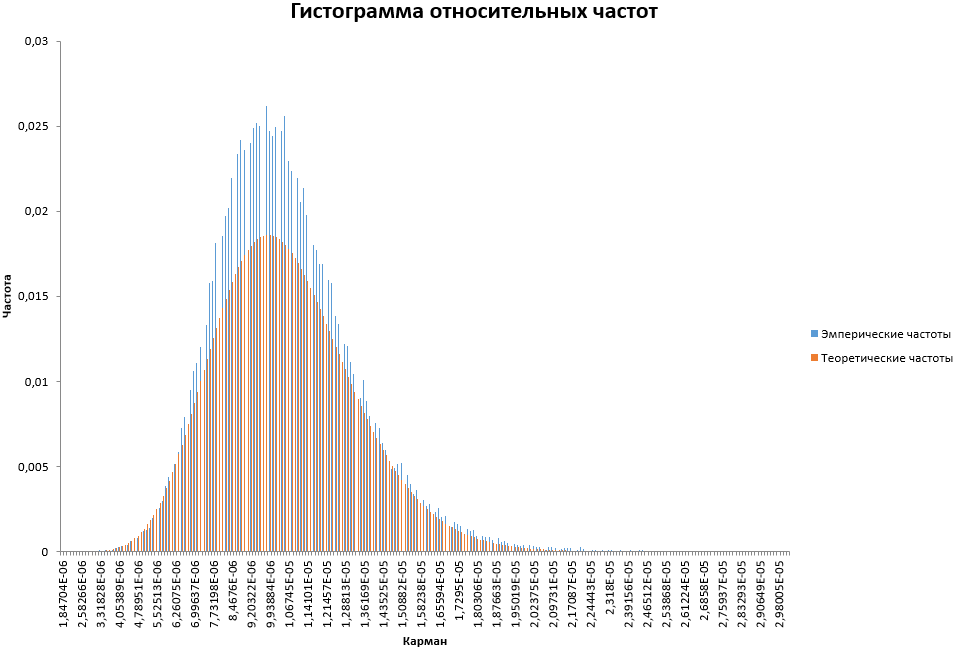
\includegraphics[width=\linewidth]{Screenshot_1.png}}
	\caption{теоретические и эмпирические частоты для алгоритма Паллоттино при $n = 80$ с разбиением нормированного сегмента [0, 1] на 232 полусегмента}
	\label{image1}
\end{figure}

\begin{figure}[!]
	\center{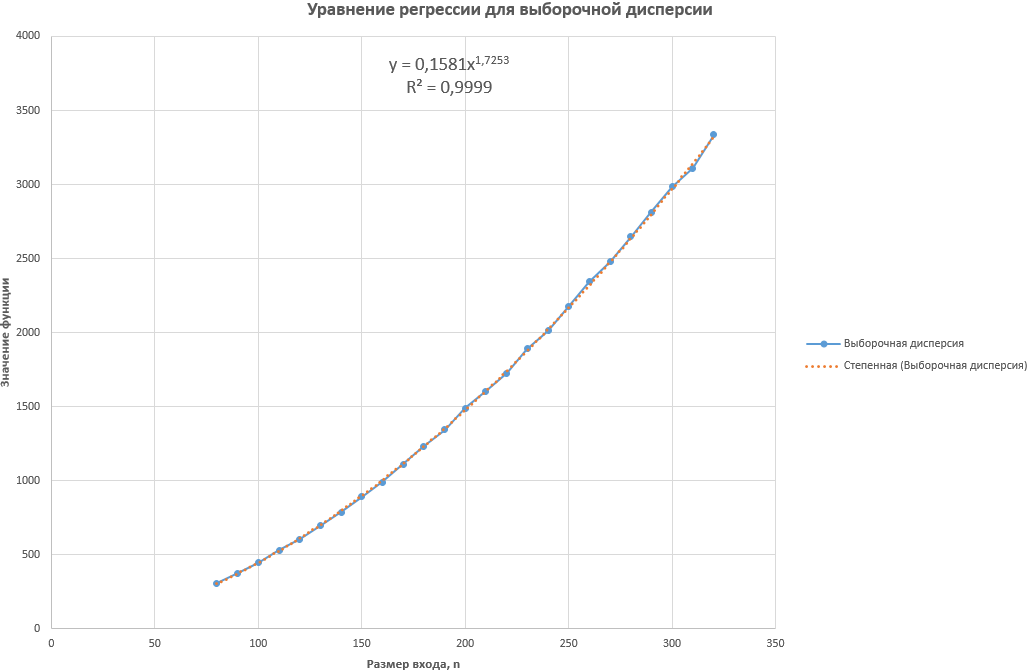
\includegraphics[width=\linewidth]{Screenshot_2.png}}
	\caption{экспериментальные данные и уравнение регрессии для выборочной дисперсии значений трудоёмкости алгоритма Паллоттино}
	\label{image2}
\end{figure}

\begin{figure}[!]
	\center{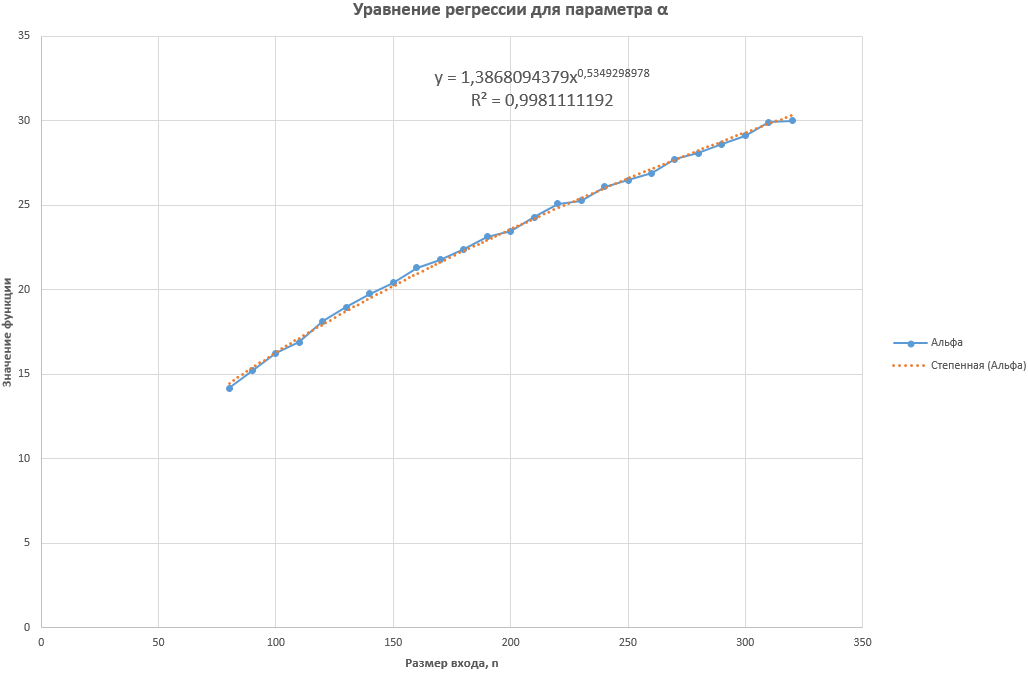
\includegraphics[width=\linewidth]{Screenshot_3.png}}
	\caption{график функции $\alpha(n)$ — параметра $\alpha$ аппроксимирующего бета-распределения для Паллоттино}
	\label{image3}
\end{figure}

\begin{figure}[!]
	\center{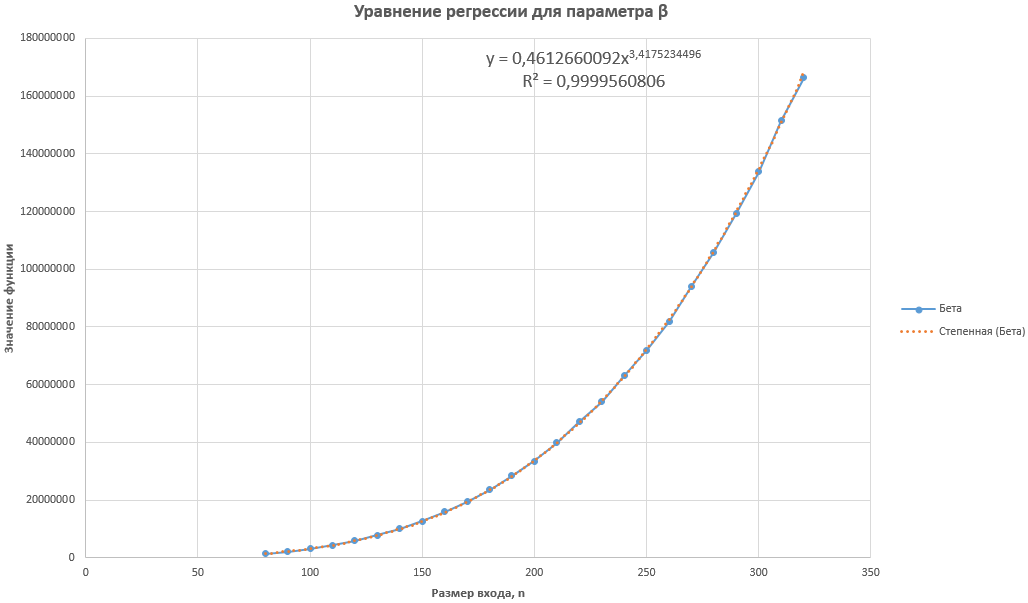
\includegraphics[width=\linewidth]{Screenshot_4.png}}
	\caption{график функции $\beta(n)$ — параметра $\beta$ аппроксимирующего бета-распределения для Паллоттино}
	\label{image4}
\end{figure}

\begin{figure}[!]
	\center{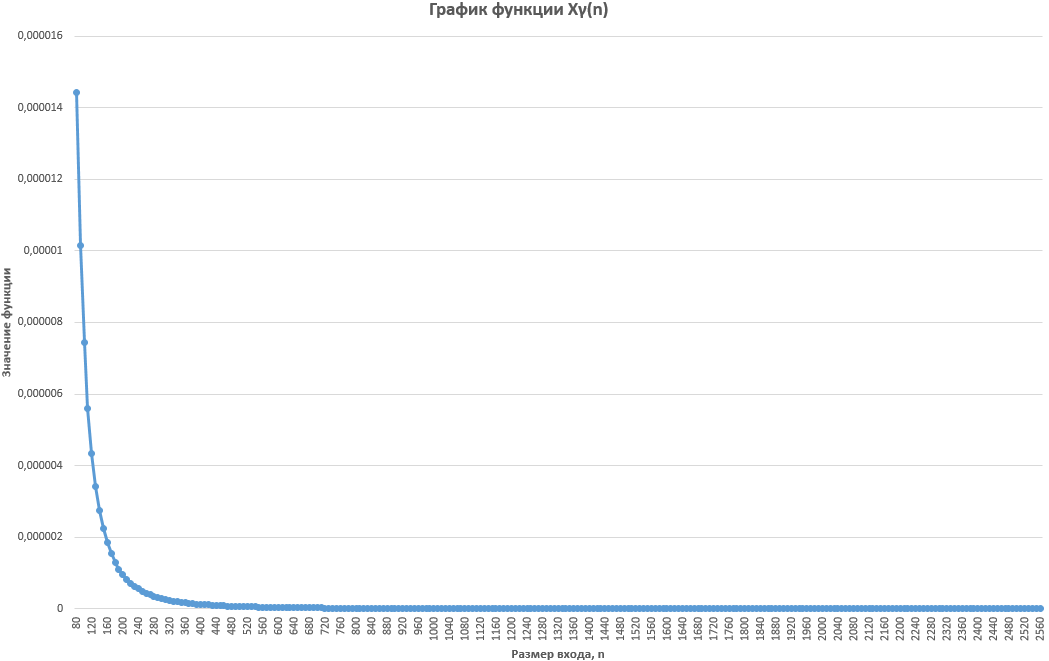
\includegraphics[width=\linewidth]{Screenshot_5.png}}
	\caption{График зависимости левого $\gamma$-квантиля бета-распределения $x_\gamma(n)$ от длины входа для алгоритма Паллоттино}
	\label{image5}
\end{figure}

\begin{figure}[!]
	\center{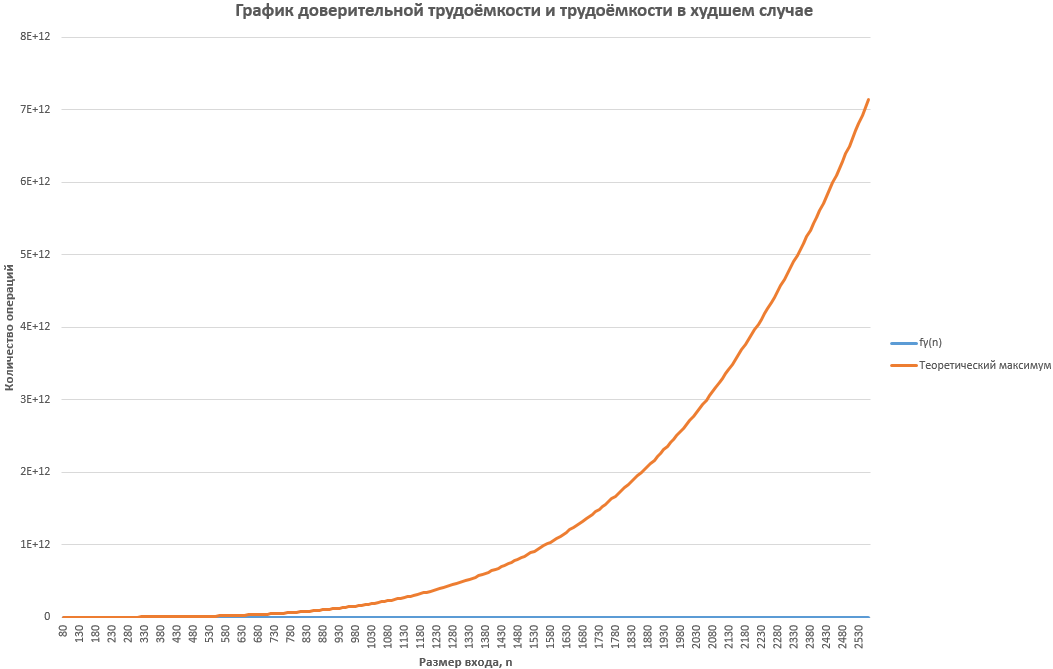
\includegraphics[width=\linewidth]{Screenshot_6.png}}
	\caption{график доверительной трудоёмкости и трудоёмкости в худшем случае для алгоритма Паллоттино}
	\label{image6}
\end{figure}

\newpage

\section{References} \label{sec:sources}

\begin{enumerate}
	\bibitem{dijkstra} E.W. Dijkstra, A note on two problems in connexion with graphs, Numer. Math. 1 (1959), 269–271.
	
	\bibitem{bellman} R. Bellman, On a routing problem, Quart. Appl. Math. 16 (1958), 87–90.
	
	\bibitem{ford} L.R. Ford and D.R. Fulkerson, Flows in Networks, Princeton University Press, Princeton, NJ, 1962.
	
	\bibitem{moore} E.F. Moore, The shortest path through a maze, volume 3523 of Bell Telephone System. Technical publications. monograph, 1959.
	
	\bibitem{desopo} M. Pollack and W. Wiebenson, Solutions of the shortest-route problem – A review, Oper. Res. 8 (1960), 224–230.
	
	\bibitem{pape} U. Pape, Implementation and efficiency of Moore-algorithms for the shortest route problem, Math. Program. 7 (1974), 212–222.
	
	\bibitem{levit_livshits} B.J. Levit and B. Livshits, Neleneinye setevye transportnye zadachi, Transport, Moscow, 1972.
	
	\bibitem{pallottino} S. Pallottino, Shortest-path methods: Complexity, interrelations and new propositions, Networks 14 (1984), 257–267.
	
	\bibitem{petrushyn_ulyanov_analysis} Петрушин В. Н., Ульянов М. В, Кривенцов А. С., Доверительная трудоемкость~--- новая оценка качества алгоритмов // Информационные технологии и вычислительные системы, 2009. №2. С.~23--37.
	
	\bibitem{petrushyn_ulyanov_planning} Петрушин В. Н., Ульянов М. В. Планирование экспериментального исследования трудоемкости алгоритмов на основе бета"=распределения // Информационные технологии и вычислительные системы, 2008. №2. С.~81--91.
	
	\bibitem{berube} P. Berube, J.N. Amaral, Combined profiling: A methodology to capture varied program behavior across multiple inputs, (2012) ISPASS 2012 - IEEE International Symposium on Performance Analysis of Systems and Software, art. no. 6189227, pp.~210--220.
\end{enumerate}

\appendix
\section{Appendix} \label{sec:appendix}

\begin{enumerate}
	\item Репозиторий проекта по анализу алгоритма Паллоттино на языке программирования C++ \\ (https://github.com/Vasar007/algorithm$\_$analysis). \label{appendix1}
\end{enumerate}

\end{document}
